\documentclass{itkmitlproject}

\usepackage{afterpage}
\usepackage{graphicx,amsmath,latexsym,amssymb,amsthm}
\usepackage{indentfirst}
\usepackage{cite}

\graphicspath{ {images/} }

\makeatletter
% \patchcmd{<cmd>}{<search>}{<replace>}{<succes>}{<failure>}
\patchcmd{\@chapter}{\addtocontents{lof}{\protect\addvspace{10\p@}}}{}{}{}% LoF
\patchcmd{\@chapter}{\addtocontents{lot}{\protect\addvspace{10\p@}}}{}{}{}% LoT
\makeatother

%1. Your thesis title (THAI)
\newcommand{\ThesisTitle}{การจัดกลุ่มข้อมูลที่ไม่มีความสมดุลกันโดยใช้การเรียนรู้เชิงลึกแบบผสม}
%2. Your thesis title (ENG)
\newcommand{\ThesisTitleENG}{Hybrid Deep Learning for Class Imbalance on Classification}
%3. Author name
\newcommand{\Author}{ธนวัฒน์ หลอดแก้ว}
%4. Author name ENG
\newcommand{\AuthorENG}{Thanawat Lodkaew}
%5. Author student ID
\newcommand{\SId}{59070071}
%9. Advisor name
\newcommand{\Advisor}{รองศาสตราจารย์ ดร. กิติ์สุชาต  พสุภา}
%10. Advisor name ENG
\newcommand{\AdvisorENG}{Assoc. Prof. Dr. Kitsucart  Pasupa}
%11. ภาคเรียนที่
\newcommand{\Sem}{1}
%12. ปีการศึกษา พ.ศ.
\newcommand{\AcaY}{2562}
%13. ปีการศึกษา ค.ศ.
\newcommand{\AcaYAD}{2019}
%14. วันส่งรายงาน
\newcommand{\SubD}{10 พฤศจิกายน พ.ศ. 2561}

\begin{document}    
    \frontmatter
    \lhead{}\rhead{}\chead{}\lfoot{}\cfoot{\thepage}\rfoot{}
    \makecover    
    \makeinnercover
    \makeengcover
    \makecopyrightcover
    \makethesiscert
    \makeprojectcert
   
    % Setting margin for page numbering on frontmatter
    \newgeometry{top=1in, bottom=1in, left=1.5in, right=1in, includefoot}
    
    \makeabstract{
        บทคัดย่อ
    }

    \makeabstracteng{
        Abstract eng
    }

    \makeack

    \newpage
    \addcontentsline{toc}{chapter}{สารบัญ}
    \tableofcontents
    
    \newpage
    \addcontentsline{toc}{chapter}{สารบัญตาราง}
    \listoftables    
    
    \newpage
    \addcontentsline{toc}{chapter}{สารบัญภาพ}
    \listoffigures
    
    % Reset frontmatter page numbering margin, back to original margin from class file
    \restoregeometry

    \mainmatter
    \lhead{}\rhead{\thepage}\chead{}\lfoot{}\cfoot{}\rfoot{}
    
    \chapter{บทนำ}
\label{chapter:introduction}

\section{ที่มาและความสำคัญ}
ในด้านการเรียนรู้ของเครื่องจักร (Machine Learning) ความไม่สมดุลกันของข้อมูล หมายถึง การที่จำนวนตัวอย่างของแต่ละกลุ่มข้อมูลมีจำนวนไม่เท่ากัน ซึ่งความไม่สมดุลกันของข้อมูลนี้ถูกนิยามให้เป็นปัญหาในการจัดกลุ่มข้อมูล (Classification) สาเหตุที่ความไม่สมดุลกันของข้อมูลเป็นปัญหา คือ อัลกอริทึมการจัดกลุ่ม (Classification Algorithm) จะทำงานได้อย่างมีประสิทธิภาพก็ต่อเมื่อจำนวนตัวอย่างของแต่ละกลุ่มข้อมูลมีจำนวนที่เท่าหรือใกล้เคียงกัน เมื่อมีความไม่สมดุลกันของข้อมูลจะทำให้การทำงานของอัลกอริทึมมีประสิทธิภาพด้อยลง ซึ่งอาจจะด้อยลงจนไม่สามารถจัดกลุ่มข้อมูลได้เลย

การจัดกลุ่มข้อมูลที่มีจำนวนตัวอย่างของแต่ละกลุ่มไม่สมดุลกันเป็นเรื่องธรรมดาอย่างมากในทางปฏิบัติ เนื่องจากข้อมูลที่เกิดขึ้นล้วนแต่ไม่สามารถคาดเดาได้อย่างแน่นอนว่าจำนวนตัวอย่างของแต่ละกลุ่มจะสมดุลกัน อีกทั้งข้อมูลส่วนใหญ่ยังมีลักษณะที่มีจำนวนตัวอย่างของแต่ละกลุ่มไม่สมดุลกัน เช่น ในระหว่างวัวอยู่ในช่วงเป็นสัด ช่วงเวลาที่วัวแสดงพฤติกรรมเป็นสัดจะมีจำนวนน้อยกว่าช่วงเวลาที่วัวไม่แสดงพฤติกรรมเป็นสัด เป็นต้น ในด้านการเรียนรู้ของเครื่องจักร มีความเป็นไปได้ว่าตัวจัดกลุ่มข้อมูลที่ถูกสร้างขึ้นจากชุดข้อมูลที่มีจำนวนตัวอย่างของแต่ละกลุ่มไม่สมดุลกันจะมีความลำเอียงในการจัดกลุ่ม กล่าวคือ มีโอกาสสูงที่ตัวจัดกลุ่มจะระบุว่าข้อมูลเป็นกลุ่มส่วนมาก (Majority Class) มากกว่าเป็นกลุ่มส่วนน้อย (Minority Class) ซึ่งเป็นผลทำให้การระบุข้อมูลเป็นกลุ่มส่วนน้อยมีความแม่นยำที่ต่ำกว่ามาตรฐาน ซึ่งความแม่นยำในการระบุข้อมูลเป็นแต่ละกลุ่มควรจะเท่าหรือใกล้เคียงกัน

ที่ผ่านมาได้มีการศึกษาเกี่ยวกับปัญหาการจัดกลุ่มข้อมูลในลักษณะนี้อย่างกว้างขวาง และได้แสดงให้เห็นถึงความสำคัญของปัญหาของการจัดกลุ่มข้อมูลที่มีจำนวนตัวอย่างของแต่ละกลุ่มไม่สมดุลกัน ซึ่งทำให้ประสิทธิภาพการจัดกลุ่มข้อมูลมีความแม่นยำที่ต่ำ ดังนั้นปัญหานี้จำเป็นต้องถูกจัดการ \cite{Buda:2017} เพื่อที่จะแก้ปัญหาการจัดกลุ่มข้อมูลที่มีจำนวนตัวอย่างของแต่ละกลุ่มไม่สมดุลกัน ได้มีเทคนิคเกิดขึ้นมากมาย โดยสามารถแบ่งเทคนิคการแก้ปัญหาได้ 2 ระดับ คือ (1) ระดับข้อมูล (Data-Level) ที่ซึ่งเป็นการแก้ปัญหาโดยการจัดการข้อมูลก่อนที่จะถูกนำไปประมวลในกระบวนการจัดกลุ่มข้อมูล โดยการสุ่มเพิ่มจำนวนตัวอย่างข้อมูล (Over-Sampling) และการสุ่มลดจำนวนตัวอย่างข้อมูล (Under-Sampling) เป็นเทคนิคในการแก้ปัญหาในระดับข้อมูล เทคนิคการแก้ปัญหาในระดับนี้เป็นการแก้ปัญหาแบบเบื้องต้นที่สามารถดำเนินการได้ง่าย อย่างไรก็ตามการสุ่มเพิ่มจำนวนตัวอย่างข้อมูลสามารถทำให้เกิดปัญหา Overfitting ตามมาได้อย่างง่ายดาย ในทางเดียวกันการสุ่มลดจำนวนตัวอย่างข้อมูลอาจจะเป็นการกำจัดสารสนเทศที่เป็นประโยชน์ต่อการจัดกลุ่มข้อมูลออกไป (2) ระดับตัวจัดกลุ่ม (Classifier-Level) ที่ซึ่งเป็นการแก้ปัญหาโดยการจัดการอัลกอริทึมการจัดกลุ่ม โดยการทำเทรสโช (Thresholding) การเรียนรู้แบบความเสียหายที่รู้สึกได้ง่าย (Cost-Sensitive Learning) การจัดกลุ่มข้อมูลแบบหนึ่งกลุ่ม (One-Class Classification) และการผนวกกันของหลายเทคนิค อย่างไรก็ตามเทคนิคเหล่านี้มียังไม่สามารถแก้ปัญหาได้อย่างมีประสิทธิภาพในทุก ๆ ชุดข้อมูล กล่าวคือ เทคนิคสามารถให้ความแม่นยำในการจัดกลุ่มข้อมูลแต่ละกลุ่มได้อย่างน่าพอใจสำหรับชุดข้อมูล A แต่ไม่สามารถทำได้อย่างมีประสิทธิภาพสำหรับชุดข้อมูล B เป็นต้น ดังนั้นเทคนิคใหม่ที่จะสามารถการแก้ปัญหาการจัดกลุ่มข้อมูลที่ไม่สมดุลกันได้อย่างมีประสิทธิภาพ และปรับเข้าได้กับทุกชุดข้อมูลจำเป็นต้องถูกคิดค้นขึ้น

\section{ความมุ่งหมายและวัตถุประสงค์ของการศึกษา}
\begin{enumerate}
	\item เพื่อศึกษาการจัดการปัญหาความไม่สมดุลกันของข้อมูลด้วยเทคนิคต่าง ๆ
	\item เพื่อศึกษาและเข้าในการทำงานของการเรียนรู้เชิงลึก (Deep Learning) อย่างท่องแท้
	\item เพื่อที่จะดัดแปลงแบบจำลองให้สามารถแก้ปัญหาความไม่สมดุลกันของข้อมูลได้
	\item เพื่อคิดค้นเทคนิคการเรียนรู้เชิงลึกแบบผสมที่สามารถจัดกลุ่มของข้อมูลได้อย่างมีประสิทธิภาพ
	\item เพื่อศึกษาความเป็นไปได้ในการประยุกต์ใช้เทคนิคที่คิดค้นกับชุดข้อมูลที่แตกต่างกัน
\end{enumerate}
\section{ขอบเขตการพัฒนาโครงงาน}
\begin{enumerate}
	\item ดัดแปลงแบบจำลองการเรียนรู้เชิงลึกให้สามารถจัดกลุ่มข้อมูลโดยไม่มีความลำเอียงกับกลุ่มส่วนมาก
	\item เปรียบเทียบประสิทธิภาพเชิงความแม่นยำของแบบจำลองที่ดัดแปลงกับเทคนิคอื่น ๆ ที่ใช้ในการแก้ปัญหาความไม่สมดุลกันของข้อมูล
\end{enumerate}
\section{ขั้นตอนการดำเนินงาน}
\begin{enumerate}
	\item ศึกษารูปแบบการแก้ปัญหาการจัดกลุ่มข้อมูลที่ไม่มีความสมดุล
	\item ศึกษาการทำงานของแบบจำลองการเรียนรู้เชิงลึก
	\item ศึกษางานวิจัยที่เกี่ยวข้อง
	\item ตั้งข้อสมมติฐาน
	\item ออกแบบแนวทางการสร้างแบบจำลองการเรียนรู้เชิงลึกแบบผสม
	\item สร้างแบบจำลองการเรียนรู้เชิงลึกแบบผสมตามที่ออกแบบ
	\item กำหนดจุดประสงค์การทดลองแต่ละแบบ
	\item ดำเนินการทำการทดลอง
	\item สรุปผลการทดลอง
\end{enumerate}
\section{ประโยชน์ที่คาดว่าจะได้รับ}
\begin{enumerate}
	\item แบบจำลองการจัดกลุ่มข้อมูลสามารถให้ความแม่นยำที่สูงในการระบุข้อมูลแต่กลุ่ม แม้ว่าจะมีความไม่สมดุลกันของข้อมูล
\end{enumerate}


    \chapter{การทบทวนวรรณกรรมที่เกี่ยวข้อง}
\label{chapter:literature-review}

\section{ทฤษฎีที่เกี่ยวข้อง}
\subsection{การเรียนรู้เชิงลึก (Deep Learning)}

\subsection{การเรียนรู้เชิงลึกแบบผสม (Hybrid Deep Learning)}
ไม่มีนิยามที่แน่นอนสำหรับแบบจำลองการเรียนรู้เชิงลึกแบบผสมว่าเป็นแบบจำลองที่มีลักษณะอย่างไร จากการศึกษาพบว่า แบบจำลองที่เกิดจากการผสมผสานกันของแบบจำลองการเรียนรู้เชิงลึกหลายสถาปัตยกรรม หรือแม้กระทั่งแบบจำลองที่มีการการคิดค้น หรือดัดแปลงฟังก์ชันสูญเสีย (Loss Function) เพื่อใช้ในการเรียนรู้ ก็สามารถเรียกได้ว่าเป็นแบบจำลองการเรียนรู้เชิงลึกแบบผสม เมื่อไม่นานมานี้ได้มีงานวิจัยพยายามคิดค้นแบบจำลองการเรียนรู้เชิงลึกแบบผสมมาเพื่อแก้ไขปัญหาต่าง ๆ และได้แสดงให้เห็นว่าแบบจำลองการเรียนรู้เชิงลึกแบบผสมนั้นมีลักษณะที่หลากหลาย Haixia Long et al. \cite{Long:2018} ได้นำเสนอสถาปัตยกรรมการเรียนรู้เชิงลึกแบบผสมสำหรับการระบุไฮดรอกซีโพรลีน (Hydroxyproline) และไฮดรอกซีไลซีน (Hydroxylysine) ในโปรตีน โดยการนำโครงข่ายประสาทแบบคอนโวลูชัน (Convolutional Neural Network: CNN) มาผนวกกับโครงข่ายประสาทแบบลองชอร์ตเทอมเมมอรี (Long Short-Term Memory: LSTM) ที่ซึ่ง CNN ถูกใช้ในการสกัดคุณลักษณะของปฏิกิริยาของกรดอะมิโน และ LSTM ถูกใช้ในการสกัดการคงอยู่ของความสัมพันธ์กันระหว่างกรดอะมิโน ผลการทดลองแสดงให้เห็นว่าสถาปัตยกรรมการเรียนรู้เชิงลึกแบบผสมนี้สามารถปรับปรุงประสิทธิภาพของแบบจำลองได้ Y. Sun et al. \cite{Sun:2016} ได้ใช้แบบจำลอง CNN หลายตัวในการสกัดคุณลักษณะสำหรับการยืนยันตัวตนด้วยใบหน้า ซึ่งคุณลักษณะของแต่ละพื้นที่ของใบหน้าจะถูกสกัดด้วยแบบจำลอง CNN ที่ต่างกัน และคุณลักษณะของแต่ละพื้นที่จถูกนำมารวมกันเพื่อจัดกลุ่ม และยืนยันตัวตนด้วยเครื่องจักรโบลทซ์มันท์แบบจำกัด (Restricted Boltzmann Machine: RBM) Jin-Young Kim et al. \cite{Jin-Young:2018} ได้คิดค้นการผสมผสานกันระหว่างโครงข่ายการสร้างข้อมูลแบบควบคุมความจริงทีแอบแฝง (Latent Semantic Controlling Generative Adversarial Network: LSC-GAN) กับตัวเข้ารหัสอัตโนมัติแบบแวริเอชัน (Variational Autoencoder: VAE) ที่ซึ่ง LSC-GAN ถูกใช้ในการสร้างข้อมูลมัลแวร์โดยอ้างอิงการแจกแจงปกติ (Gaussian Distribution) ของข้อมูลมัลแวร์จริง โดยข้อมูลจริงจะถูกนำไปแปลงให้อยู่ในรูปแบบแอบแฝง (Latent Space) ด้วย VAE เพื่อการสกัดคุณลักษณะและถูกนำไปใช้ต่อโดย LSC-GAN

งานวิจัยดังกล่าวข้างต้นแสดงให้เห็นว่าแบบจำลองการเรียนรู้เชิงลึกแบบผสมนั้นมีความหลากหลาย และมีประสิทธิภาพที่ดีกว่าแบบจำลองธรรมดา ดังนั้น ผู้จัดทำจึงเกิดความคิดที่จะคิดค้นแบบจำลองการเรียนรู้เชิงลึกแบบผสมมาเพื่อแก้ปัญหาการจัดกลุ่มข้อมูลที่ไม่มีความสมดุล

\subsection{งานวิจัยที่เกี่ยวข้อง}
เมื่อเทคนิคการจัดกลุ่มข้อมูลที่ประกอบด้วยโครงข่ายประสาทแบบคอนโวลูชันถูกใช้กับชุดข้อมูลที่มีความไม่สมดุลกัน อัตราการพยากรณ์ผิดพลาดจะมีค่าสูงเมื่อเทียบกับการเพิ่มขึ้นของจำนวนรอบของการเรียนรู้ของแบบจำลอง กล่าวคือ ยิ่งจำนวนรอบของการเรียนรู้สูงขึ้น จะทำให้อัตราการพยากรณ์ผิดพลาดสูงขึ้นด้วย \cite{Yan:2015} เบื้องหลังของสาเหตุที่ทำให้เป็นเช่นนั้น คือ ในเสตจของการเรียนรู้ของแบบจำลองการเรียนรู้เชิงลึก ข้อมูลจะถูกแบ่งออกเป็นกลุ่ม ๆ ซึ่งทำให้แต่ละกลุ่มมีความไม่เท่าเทียมกันเมื่อข้อมูลไม่สมดุลกัน อีกทั้งบางกลุ่มอาจจะมีแค่ตัวอย่างของกลุ่มข้อมูลที่เป็นส่วนมาก หรือกลุ่มข้อมูลที่เป็นส่วนน้อยเท่านั้น เมื่อแบบจำลองได้เรียนรู้ข้อมูลจากกลุ่มเหล่านั้นในทุก ๆ รอบ จึงทำให้เกิดอัตราการพยากรณ์ผิดพลาดที่สูง

เมื่อไม่นานมานี้ได้มีงานวิจัยที่พยายามจัดการกับปัญหาการเรียนรู้ของแบบจำลองการเรียนรู้เชิงลึกเมื่อต้องเรียนรู้ข้อมูลที่มีความไม่สมดุลกัน ดังต่อไปนี้

\begin{itemize}
  \item S. Wang et al. \cite{Wang:2016} ได้ทำการดัดแปลงฟังก์ชันสูญเสียอย่าง ค่าเฉลี่ยของกำลังสองของความคลาดเคลื่อน (Mean Square Error: MSE) เพื่อทำให้การเรียนรู้ของแบบจำลองกาเรียนรู้เชิงลึกไม่มีความลำเอียงในการจดจำข้อมูลที่เป็นกลุ่มส่วนมากเกินไป โดยฟังก์ชันสูญเสียใหม่นี้มีชื่อว่า ค่าเฉลี่ยของความคลาดเคลื่อนของความผิดพลาด (Mean False Error: MFE) แต่ประสิทธิภาพของฟังก์ชันสูญเสียนี้ยังไม่เป็นที่น่าพอใจ ผู้จึงได้นำเสนอ ค่าเฉลี่ยของกำลังสองของความคลาดเคลื่อนของความผิดพลาด (Mean Square False Error: MSFE) ที่ซึ่งเนการปรับปรุงความสามารถของ MFE อย่างไรก็ตามฟังก์ชันสูญเสียดังกล่าวยังไม่สามารถประยุกต์ใช้ได้กับ โครงข่าวความเชื่อแบบลึก (Deep Belief Network) และโครงข่ายประสาทแบบคอนโวลูชัน
\end{itemize}
    \chapter{วิธีการดำเนินการวิจัย}
\label{chapter:experiment}

\section{ข้อสมมติฐาาน}
สมมติฐานของงานวิจัยนี้ คือ แบบจำลองการเรียนรู้เชิงลึกที่นำเสนอจะสามารถจัดการปัญหาความไม่สมดุลกันของข้อมูลได้อย่างมีประสิทธิภาพ

\section{การทำการทดลอง}
\subsection{ชุดข้อมูล}
เพื่อที่จะได้ผลการทดลองที่สามารถเปรียบประสิทธิภาพของเทคนิคการแก้ปัญหา จำเป็นจะต้องใช้ชุดข้อมูลที่หลากหลาย โดยแบ่งออกเป็นชุดข้อมูลที่มีความสมดุลและไม่สมดุลกันของข้อมูล ดังนี้

\begin{itemize}
  \item CelebFaces Attributes Dataset (CelebA) \cite{dataset:celebA} ชุดข้อมูลนี้มีความไม่สมดุลกันของข้อมูล ที่ซึ่งเป็นชุดข้อมูลขนาดใหญ่ที่ประกอบไปด้วยภาพหน้าของคนมีชื่อเสียงกว่า 1 หมื่นคน และมีจำนวนภาพมากกว่า 2 แสนภาพ โดยภาพจะมีลักษณะเป็นท่าทางของหน้าและพื้นหลังที่หลากหลายดังรูปที่ \ref{fig:dataset:celebA-1} CelebA นั้นมีคำอธิบายประกอบ (Annotation) ที่หลากหลายมาก เช่น คำอธิบายประกอบที่บอกว่าคนในภาพคือใคร และกำลังยิ้มอยู่หรือไม่ เป็นต้น
  
\begin{figure}[h]
    \centering
    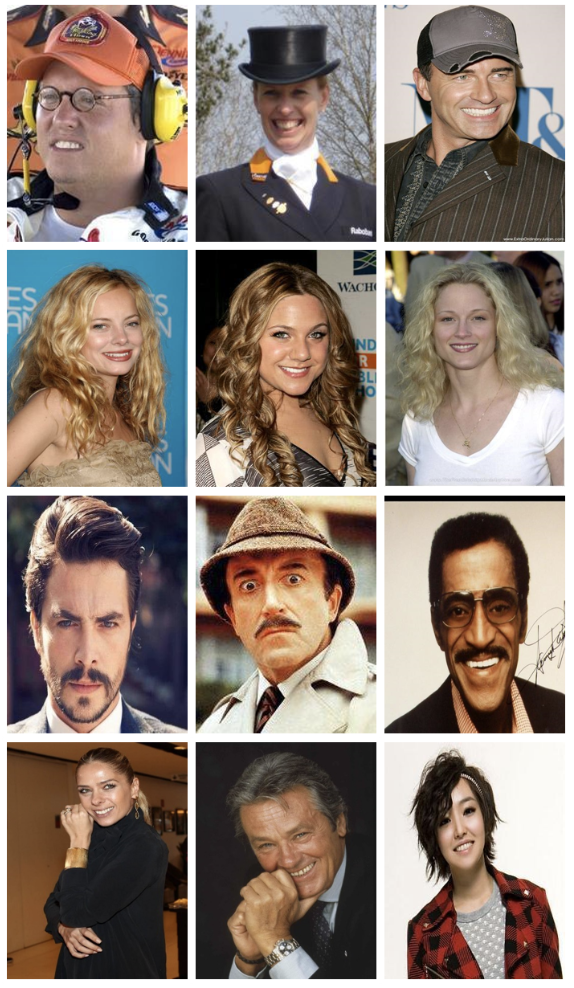
\includegraphics[scale=0.5]{celebA-1}
    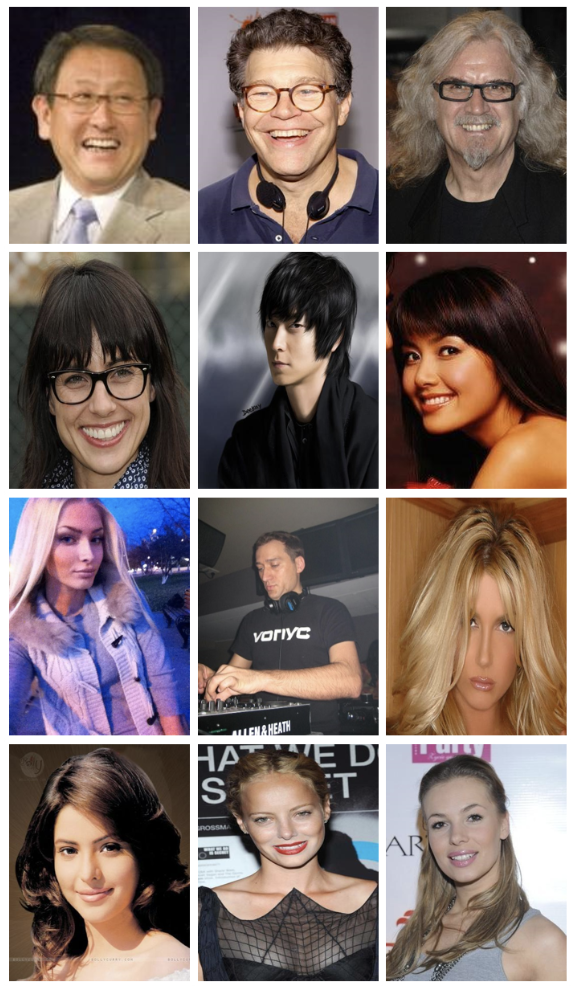
\includegraphics[scale=0.5]{celebA-2}
    \caption{ภาพตัวอย่างของชุดข้อมูล CelebA}
    \label{fig:dataset:celebA-1}
\end{figure}

  \item Cow \cite{dataset:cow} ชุดข้อมูลนี้มีความไม่สมดุลกันของข้อมูล ที่ซึ่งเป็นชุดข้อมูลประเภทวิดีโอ ที่ซึ่งแสดงการเป็นอยู่ของวัวในคอก โดยชุดข้อมูลถูกเก็บจากคอกวัวภายในฟาร์มโชคชัยด้วยกล้องวิดีโอ วิดีโอได้ถูกนำมาแปลงเป็นภาพเฟรม โดยภาพจะมีลักษณะเป็นภาพที่ถ่ายจากมุมบนดังรูปที่ \ref{fig:dataset:cow-1} คำอธิบายประกอบสำหรับชุดข้อมูลนี้ คือ การแสดงพฤติกรรมเป็นสัดของวัวแต่ละตัวในแต่ละเฟรม เช่น ในเฟรมที่ 5 วัว A แสดงพฤติกรรมเป็นสัด วัว B ไม่แสดงพฤติกรรมเป็นสัด และวัว C แสดงพฤติกรรมเป็นสัด เป็นต้น โดยจำนวนเฟรมที่วัวแต่ละตัวไม่แสดงพฤติกรรมเป็นสัดมีจำนวนมากกว่าที่แสดงพฤติกรรมเป็นสัด
  
  \begin{figure}[h]
    \centering
    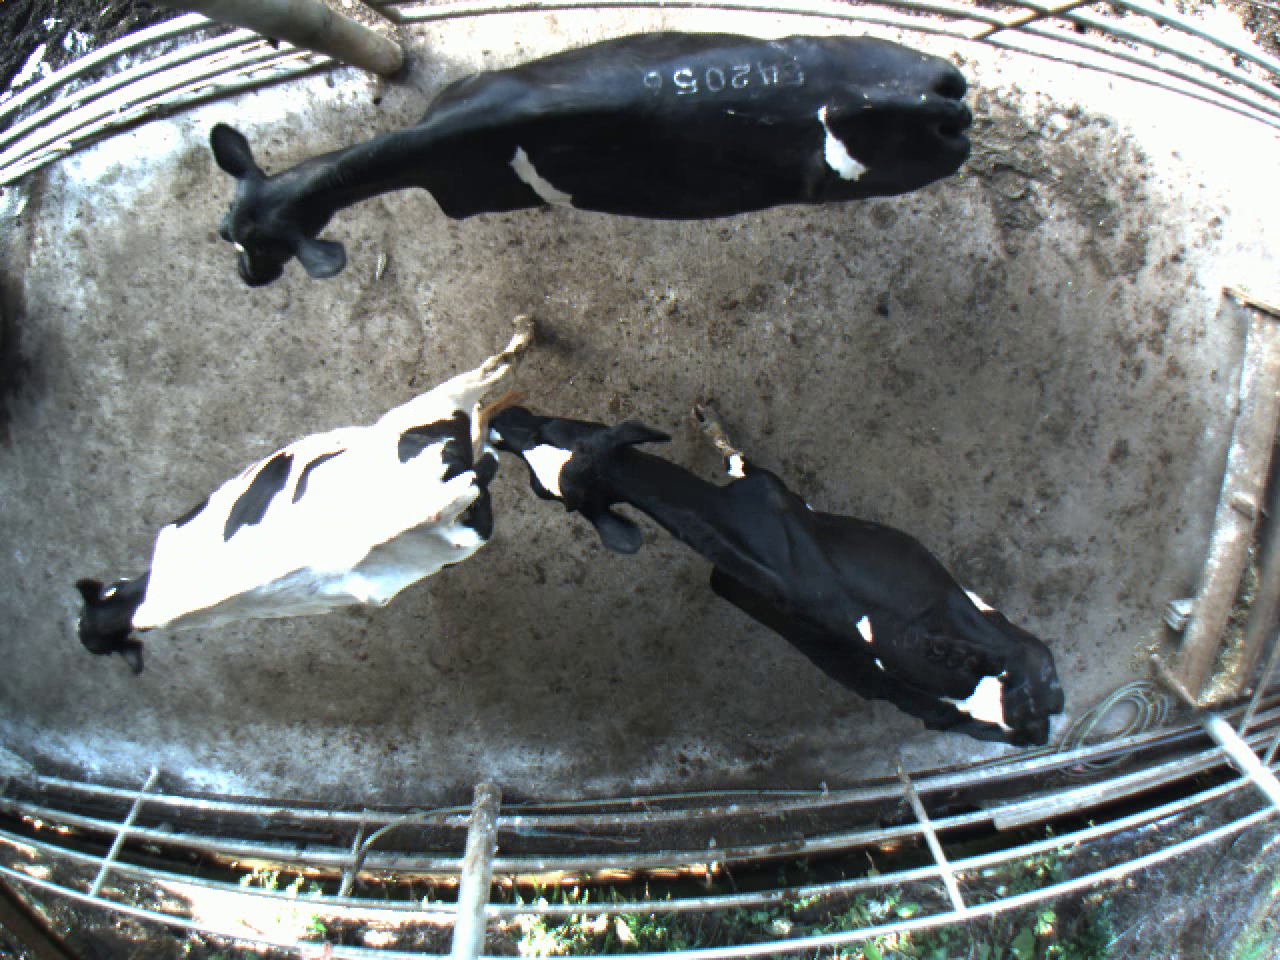
\includegraphics[scale=0.25]{cow-1}
    \caption{ภาพตัวอย่างของชุดข้อมูล Cow}
    \label{fig:dataset:cow-1}
\end{figure}

  \item CIFAR-10 \cite{dataset:cifar-10} ชุดข้อมูลนี้มีความสมดุลกันของข้อมูล ที่ซึ่งเป็นชุดข้อมูลที่ประกอบไปด้วยภาพของสัตว์และยานพาหนะดังรูปที่ \ref{fig:dataset:cifar-1} โดยแบ่งออกเป็นยานพาหนะ 4 ประเภท คือ เครื่องบิน รถยนต์ เรือ และรถบรรทุก และสัตว์ 6 ประเภท คือ นก แมว กวาง หมา กบ และม้า ซึ่งแต่ละประเภทมีจำนวน 6,000 ภาพเท่ากัน รวมทั้งหมดเป็น 6 หมื่นภาพ คำอธิบายประกอบของชุดข้อมูลนี้ คือ ประเภทของภาพ
  
    \begin{figure}[h]
    \centering
    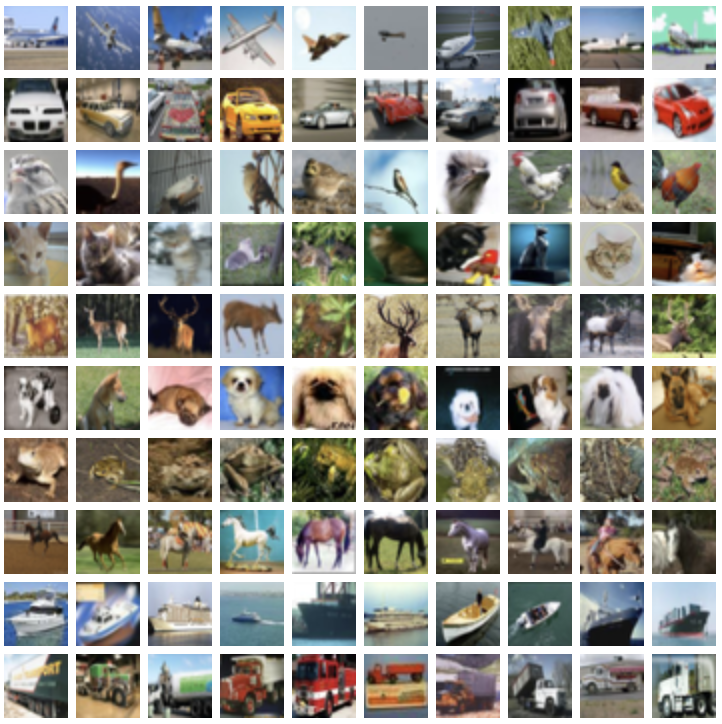
\includegraphics[scale=0.9]{cifar-1}
    \caption{ภาพตัวอย่างของชุดข้อมูล CIFAR-10}
    \label{fig:dataset:cifar-1}
\end{figure}

\end{itemize}

    \chapter{ผลการทดลองเบื้องต้น}
\label{chapter:result}

บทที่สี่
    \include{chapter5}
    
    \clearpage
    \addcontentsline{toc}{chapter}{บรรณานุกรม}
    \bibliographystyle{IEEEtran}
    \bibliography{reference}
    
    \startappendix
    \include{appendix}
    
\end{document}